\Section{Algorithm Description}
\label{MG:Sec:DGCNN}

Our work on applying DGCNN for malware classification in \sysname has been inspired by the deep learning model proposed in~\cite{Dgcnn}. In this section, we first introduce how DGCNN aggregates attributes through the neighborhood defined by the graph structure. We then discuss how to extend the existing DGCNN model with our own modifications. To explain the rationale of the DGCNN-based malware classification algorithm clearly, we walk through an example graph with five vertices as shown in Figure~\ref{MG:Fig:ExampleGraph}.

\Subsection{Primer on DGCNN}

\paragraphb{Notations.} We denote the adjacency matrix of a graph $G=(V, E)$ of $n$ vertices as $\mathbf{A} \in \mathbb{Z} ^{n\times n}$.
Note that $G$ is a directed graph, and $\mathbf{A}$ is not necessarily symmetric.
To allow the attributes of a vertex to be propagated back to the vertex itself, we define the augmented adjacency matrix $\tilde{\mathbf{A}} = \mathbf{A} + \mathbf{I}$.
Accordingly, the augmented diagonal degree matrix of $G$ is defined as $\tilde{\mathbf{D}}$, where
$\tilde{\mathbf{D}}_{i,i} = \sum_j \tilde{\mathbf{A}}_{i,j}$.
We assume that each vertex is associated with a $c$-dimension attribute vector.
Therefore, we use $\mathbf{X} \in \mathbb{R}^{n \times c}$ to denote the attribute matrix for all the vertices in the graph. %$\forall v \in V$.
Alternatively, we can also treat $\mathbf{X}$ as the concatenation of $c$ \textit{attribute channels} of the graph.
For the sample graph $g$ in Figure~\ref{MG:Fig:ExampleGraph}, we assume the vertices have two attribute channels,
and display the corresponding augmented adjacency matrix $\tilde{\mathbf{A}}$, the augmented diagonal degree matrix $\tilde{\mathbf{D}}$,
and the attribute matrix $\mathbf{X}$ with two attribute channels named $F1$ and $F2$.
Given $\tilde{\mathbf{A}}$ and $\mathbf{X}$ for graph $G$, the DGCNN-based algorithm performs three sequential stages to obtain its tensor representation for malware classification. Note that $\tilde{\mathbf{D}}$ can be calculated from $\tilde{\mathbf{A}}$.

\begin{figure*}[htbp]
    \centerline{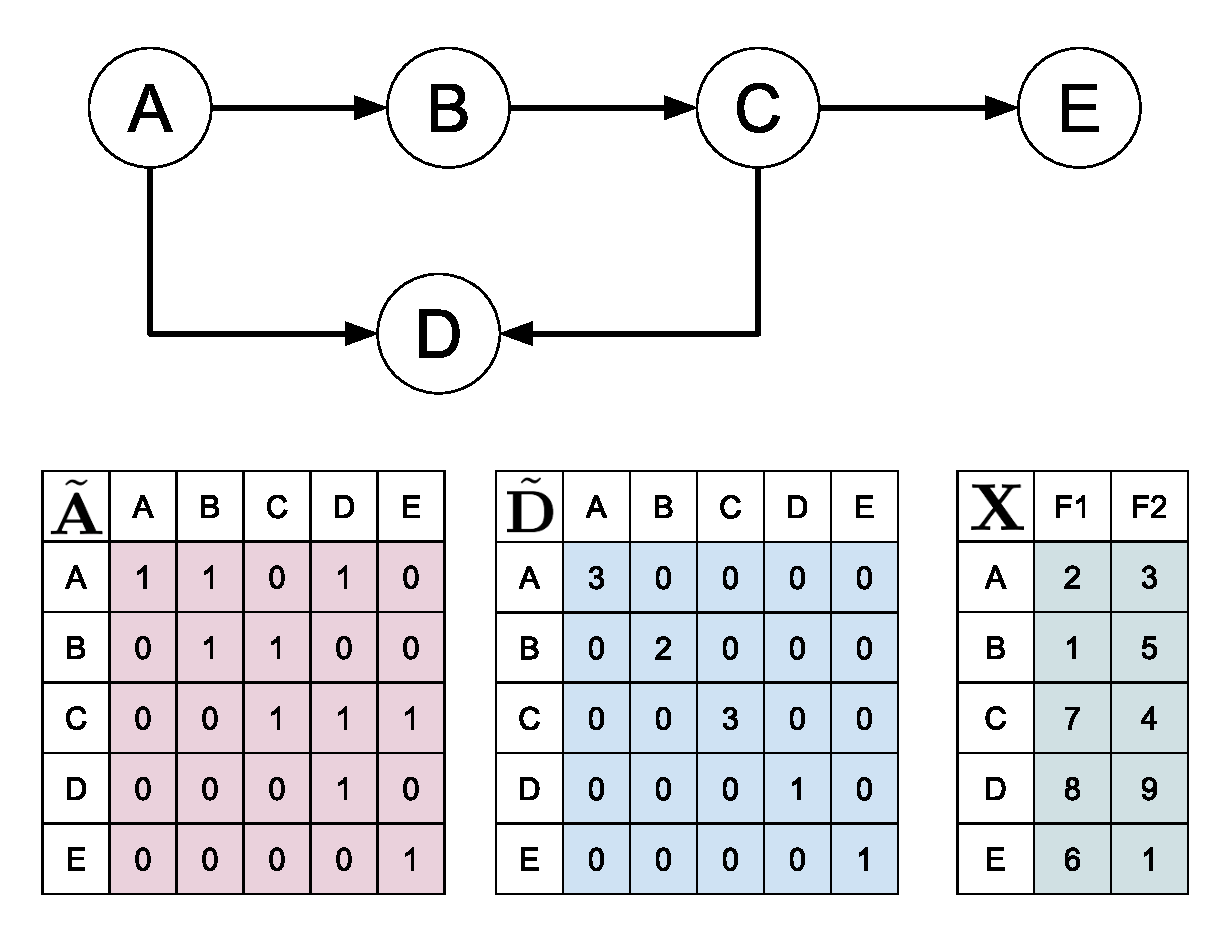
\includegraphics[width=0.90\textwidth]{Magic/figures/ExampleGraph.eps}}
    \caption{An Example Graph $g$ and its Corresponding Matrices}
    \label{MG:Fig:ExampleGraph}
\end{figure*}

\paragraphb{Graph Convolution Layer(s).} In the first stage, a \textit{graph convolution} technique propagates each vertex's attributes to its neighborhood based on the structural connectivity.
To aggregate multi-scale sub-structural attributes, multiple graph
convolution layers are stacked, which can be defined recursively as follows:
\begin{equation}
    \mathbf{Z}^{t + 1} = f(\tilde{\mathbf{D}}^{-1} \tilde{\mathbf{A}} \mathbf{Z}^t \mathbf{W}^t)
\end{equation}
where $Z^0 = X$. The $t$-th layer takes input $Z^t \in \mathbb{Z}^{n \times c_t}$,
mapping $c_t$ feature channels into $c_{t+1}$ feature channels with the graph convolution parameter $\mathbf{W}^t \in \mathbb{R}^{c_t \times c_{t+1}}$.
The newly obtained channels of each vertex are then propagated to both its neighboring vertices and itself,
 first multiplied with the augmented adjacency matrix $\tilde{\mathbf{A}}$,
and then normalized row-wisely using the augmented degree diagonal matrix $\tilde{\mathbf{D}}$.
This key step enables vertices to pass its own attributes through the graph in a breadth-first-search fashion. %It can be explained as follows.
Define $\mathbf{F} = \mathbf{Z}^t \cdot \mathbf{W}^t$ and $\mathbf{O} = \tilde{\mathbf{A}} \cdot \mathbf{F}$, where
\begin{align}
    \mathbf{O}[i][j] &= \sum_{k = 1}^{n} \tilde{\mathbf{A}}[i][k] \times \mathbf{F}[k][j]
\end{align}
$\forall 1\leq i \leq n, 1 \leq j \leq c_t$.
In other words, the $j$-th feature channel of vertex $i$ is computed as a linear combination of all its neighbors' $j$-th feature channels.
The layer finally outputs the element-wise activation using a nonlinear function $f$.
At the end of $h$ graph convolution layers, DGCNN concatenates each layer's output $Z^{t}$,
denoted as $\mathbf{Z}^{1:h} = [\mathbf{Z}^1, \mathbf{Z}^2, \ldots, \mathbf{Z}^{h}]$.
For the sample graph $g$, Figure~\ref{MG:Fig:ExampleGraphConvolution} shows how the two sequential graph convolution layers transform the initial attribute matrix $\mathbf{Z}_0=\mathbf{X}$ to $\mathbf{Z}_1$ and $\mathbf{Z}_2$, both of which together form $\mathbf{Z}^{1:2}$.
After applying $h=2$ graph convolution layers, the sample graph $g$ is transformed to $\mathbf{Z}^{1:h}$.
We assume the weight parameters in the two graph convolution layers are $\mathbf{W}^1 = [[1, 0 ,1], [0, 1, 0]]$ and $\mathbf{W}^2 = [[0, 1 ,-2, 2], [1, 1, 7, -2], [1, 0, -1, 4]]$.
For simplicity, numbers are of 2 precision, and we perform the element-wise RELU nonlinear activation $f(x) = max(x, 0)$ in both graph convolution layers.

\begin{figure*}[htbp]
    \centerline{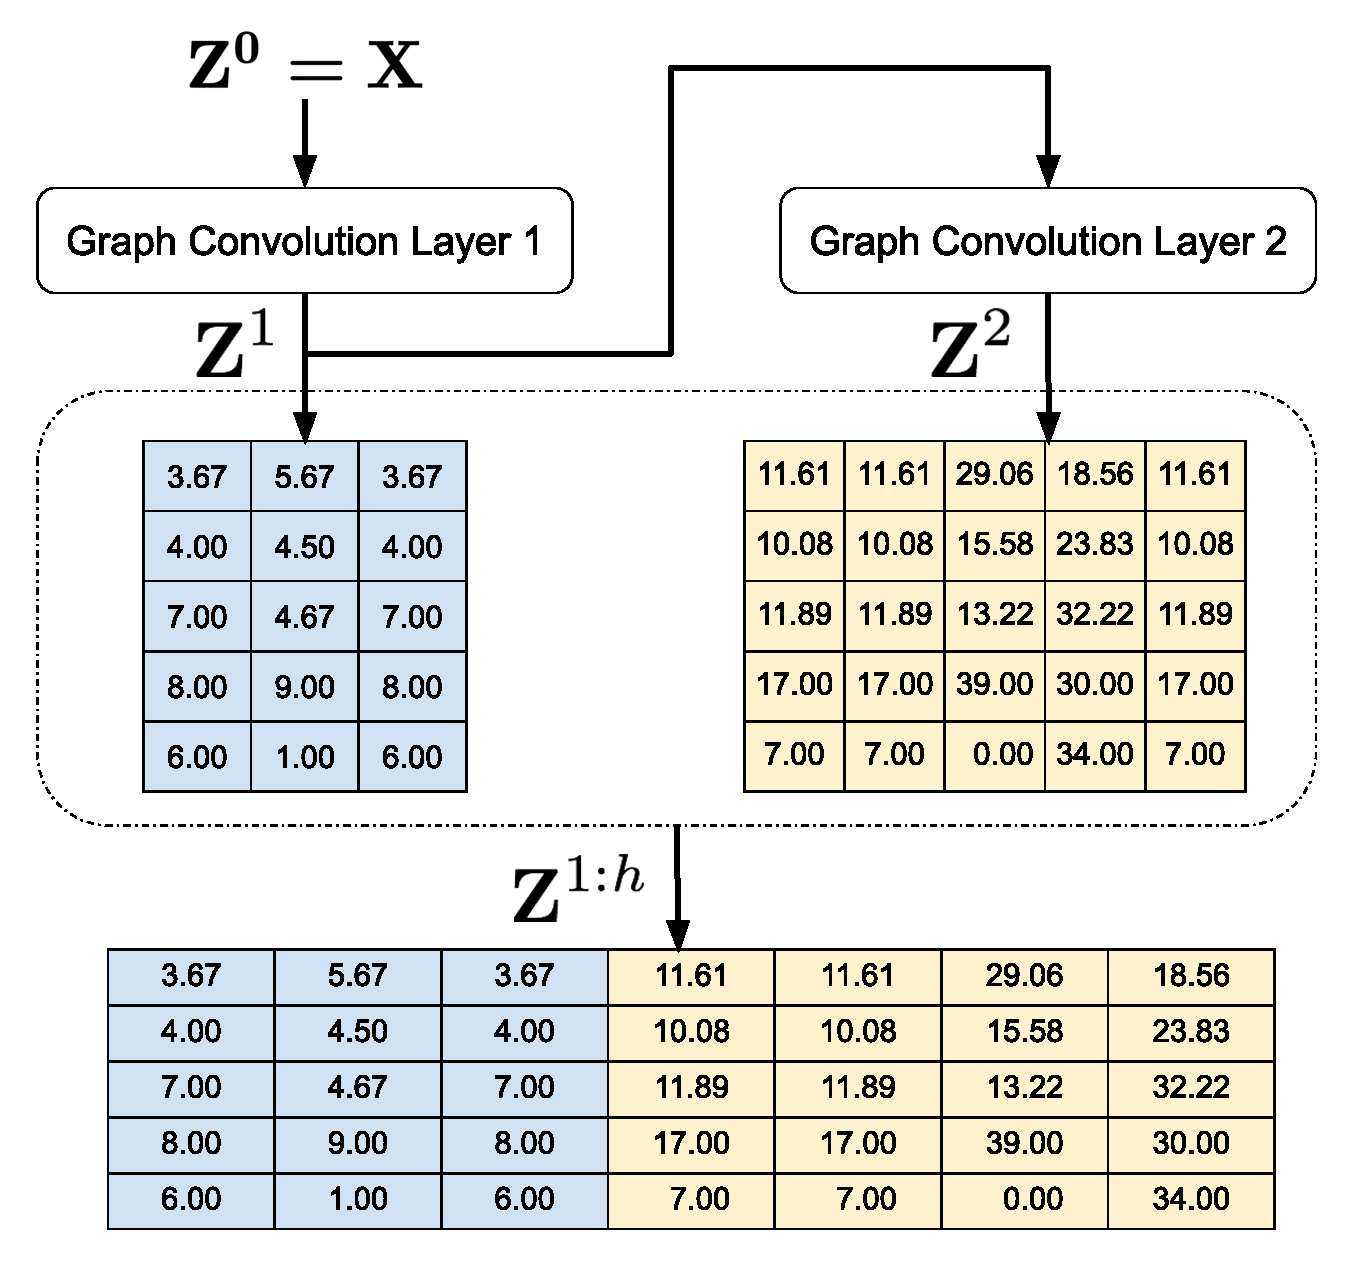
\includegraphics[width=0.90\textwidth]{Magic/figures/ExampleGraphConvolution.eps}}
    \caption{Applying $h=2$ Graph Convolution Layers to Example Graph $g$}
    \label{MG:Fig:ExampleGraphConvolution}
\end{figure*}

\paragraphb{SortPooling Layer.} Intuitively $\mathbf{Z}^{1:h}$ has $n$ rows and $\sum_{1}^{h}c_t$ column,
which corresponds to the \textit{feature descriptor} of each vertex at different scales.
The second stage, namely the \textit{sortpooling} layer,
leverages the feature descriptors to sort the vertices.
Vertices in different graphs will be put in similar positions as long as they have similar weighted feature descriptors.
The sortpooling layer starts with the last layer because $\mathbf{Z}^{h}$ is approximately
equivalent to the most refined continuous colors as in the Weisfeiler-Lehman graph kernels~\cite{WlGraphKernel}.
More specifically, vertices are first sorted by the last channel of the last layer in a decreasing order.
%When a tie on the last channel occurs, sorting will use the second last channel.
If there are $c_h$ ties on the last layer's output $\mathbf{Z}^{h}$,
sorting continues by using the second last layer's output $\mathbf{Z}^{h - 1}$, and the procedure repeats until all ties are broken.
The sortpooling layer further truncates or pads the sorted tensors by the first dimension so that it outputs $\mathbf{Z}^{sp}$ of size $k$ by $\sum_{1}^{h}c_t$.
Hence, the sortpooling process unifies the size of feature descriptors for all graphs.
Following our sample graph $g$, we visualize this process in Figure~\ref{MG:Fig:ExampleSortpool}.
Given the graph convolution result $\mathbf{Z}^{1:h}$ for the sample graph $g$ in Figure~\ref{MG:Fig:ExampleGraphConvolution},
the sortpooling layer with $k = 3$ sorts the feature descriptors (based on only the last feature channel in this example) and then truncates the two `smallest' rows.
The row of $\mathbf{Z}^{h}$ is first sorted using only the value in the last column.
The last two rows (i.e., yellow and red) are discarded from the sorted matrix as $n - k = 2 > 0$.

\paragraphb{Remaining Layer(s).} In the last stage,
the authors of the original DGCNN\cite{Dgcnn} append a one-dimension convolution (Conv1D) layer of kernel size $\sum_{1}^{h}c_t$ and stride size $\sum_{1}^{h}c_t$.
If $F$ is the number of filters in the last one-dimension convolution layer,
the sort pooling output $\mathbf{Z}^{sp}$ will be reduced to a one-dimension vector of size $k \times F$,
which is then fed into a fully connected one-layer perceptron for graph classification.

\begin{figure*}[htbp]
    \centerline{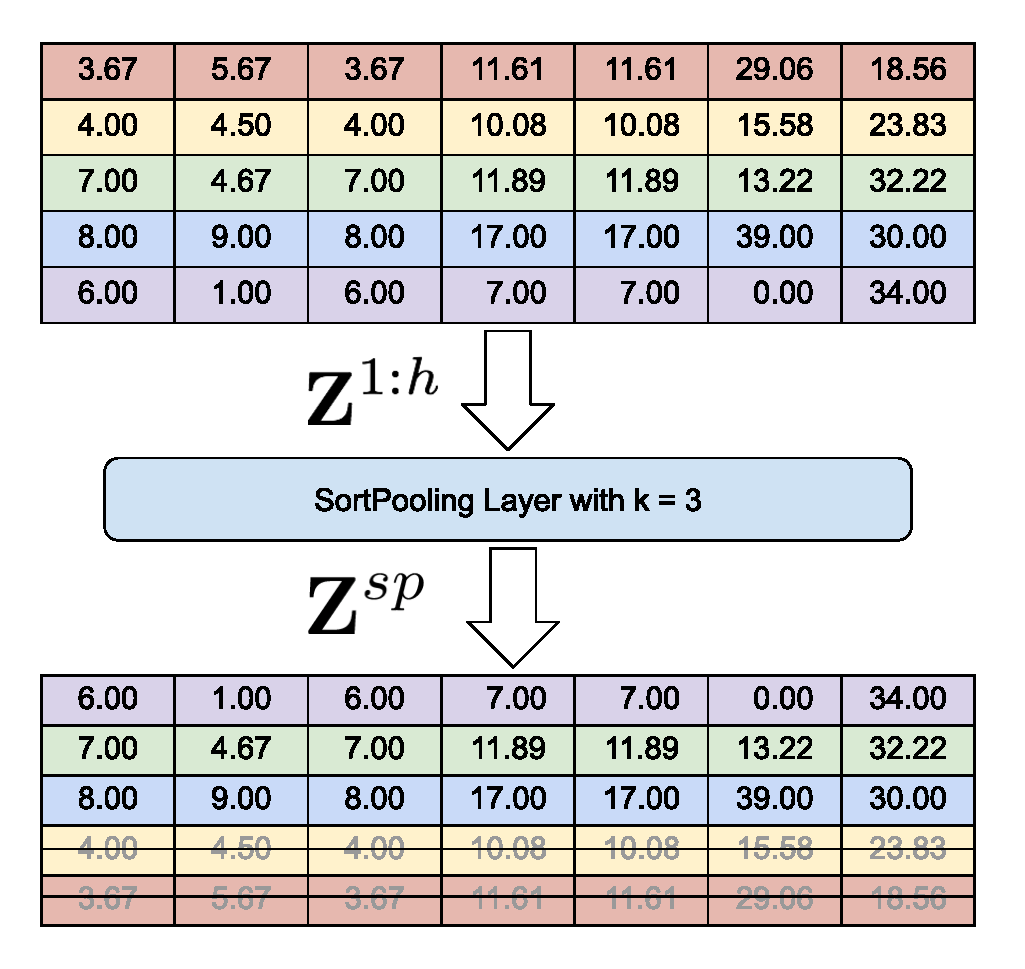
\includegraphics[width=0.90\textwidth]{Magic/figures/ExampleSortpool.eps}}
    \caption{Applying Sortpooling Layer to Example Graph $g$}
    \label{MG:Fig:ExampleSortpool}
\end{figure*}

\Subsection{WeightedVertices Layer}
In the first extension to DGCNN, we observe that the Conv1D layer following the sortpooling layer can alternatively be of kernel size $k$, stride size $k$, and single channel.
Mathematically, a single channel Conv1D layer can be represented as a row of parameters $W \in \mathbb{R}^{1 \times k}$.
Its output $E \in \mathbb{R}^{1 \times \sum_{1}^{h}c_t}$, when fed with \textit{transposed} $\mathbf{Z}^{sp}$, will be equivalent to
\begin{equation}
    E = f(\mathbf{W} \times \mathbf{Z}^{sp})
    \label{MG:Equ:WeightedVertices}
\end{equation}
%which is obviously after we notice that
This is because
\begin{equation}
    E_c = f(\sum_{i}^{k} W_i \times \mathbf{Z}^{sp}_{i, c})
\end{equation}
where $1\leq c \leq \sum_{1}^{h}c_t$, and $f$ is an element-wise nonlinear activation function.
Inspired by the graph embedding idea in\cite{GraphEmbedding}, our Conv1D layer treats each row of the sort pooling result $\mathbf{Z}^{sp}_{i}$ as the embedding of the vertices kept by the sortpooling layer.

Equivalently, Equation~(\ref{MG:Equ:WeightedVertices}) computes $E$, the embedding of the graph obtained through a weighted summation of vertex embeddings \cite{GraphEmbedding}.
For our sample graph $g$, its ``embedding" is computed in Figure~\ref{MG:Fig:ExampleWeightedVertice}, where we assume weight vector $\mathbf{W}=[0.4, 0.1, 0.5]$.
WeightVertices layer aggregates sample graph $g$'s vertex embeddings,
e.g. the output of sort pooling layer $\mathbf{Z}^{sp}$ in Figure~\ref{MG:Fig:ExampleSortpool}, to graph embedding $E$.
We choose again RELU as the nonlinear activition function $f$ for simplicity.
In reality, $\mathbf{W}$ is updated by gradient descent during the process of minimizing the classification loss.
For ease of presentation, in the remainder of the paper we refer to this special Conv1D layer after the sortpooling layer as the \textit{WeightedVertices} layer.
We replace the original Conv1D layer with the WeightVertices layer, because the WeightVertices layer leverages the graph embedding idea to make the output from the sorting pooling layer compatible with the malware classifier.

\begin{figure*}[htbp]
    \centerline{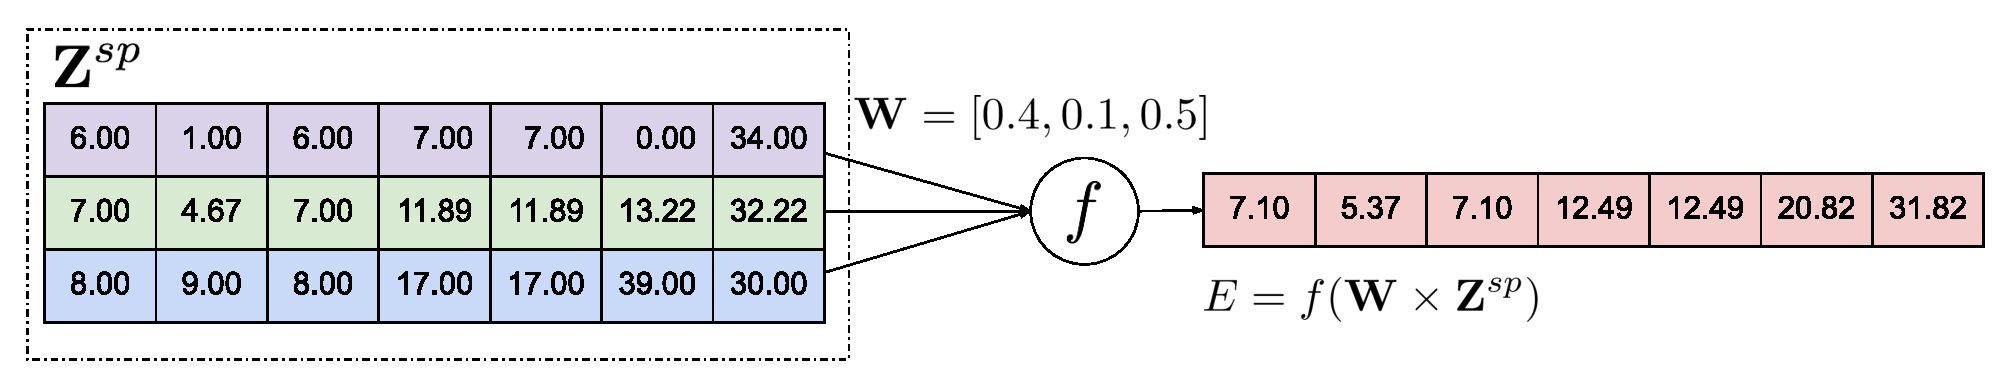
\includegraphics[width=0.90\textwidth]{Magic/figures/ExampleWeightedVertice.eps}}
    \caption{Applying WeightVertices Layer to Example Graph $g$}
    \label{MG:Fig:ExampleWeightedVertice}
\end{figure*}

\Subsection{AdaptiveMaxPooling: An Alternative to Sortpooling}
The intuition behind sorting from the deeper layer is to treat its output as more refined WL colors\cite{WlAlgorithm, WlGraphKernel}.
The inner sorting inside the channels of a fixed layer output is, however, less reasonable.
Besides, the Conv1D addendum is only aggregating the feature descriptors of per vertex and per convolution channel separately.

Our second extension is to apply the adaptive max pooling (AMP) on the concatenated graph convolution layer output $\mathbf{Z}^{1:h}$.
Given an set of two-dimension inputs of various sizes $\{x_i | x_i \in \mathbb{R}^{h_i \times w_i}\}$,
The AMP layer divides each input $x_i$ into a $H \times W$ grid with a sub-window size approximately to $h_i / H$ and $w_i / W$,
and then automatically chooses kernel sizes as well as convolution strides for different $x_i$.
Inside each sub-window and each channel, only the maximum element is kept in order to form the set of identical-dimension outputs $\{y_i | y_i \in \mathbb{R}^{ H \times W}\}$.
The way in which AMP works for our sample graph $g$ is illustrated in Figure~\ref{MG:Fig:ExampleAmp}.
The left top matrix $\mathbf{Z}^{1:h}_g$ represents the graph convolution output of the sample graph $g$ in Figure~\ref{MG:Fig:ExampleGraph}.
The left bottom matrix $\mathbf{Z}^{1:h}_{g'}$ represents the graph convolution output of another imaginary graph $g'$ with four vertices.
For $\mathbf{Z}^{1:h}_g$ of size $5\times 7$, adaptive max pooling's kernel size = $3 \times 3$ (shown as red shadow).
For $\mathbf{Z}^{1:h}_{g'}$ of size $4\times 7$, adaptive max pooling's kernel size = $2 \times 3$ (shown as red shadow).
For both inputs, padding = 0, stride = $2 \times 1$.
Since the dimension of the graph convolution output $\mathbf{Z}^{1:h}_g$ for $g$ is $5 \times 7$, AMP uses a max pooling kernel of size $3 \times 3$.
To show how AMP works for inputs of different dimension sizes, in Figure~\ref{MG:Fig:ExampleAmp} we also feed $\mathbf{Z}^{1:h}_{g'}$,
the graph convolution output for another graph $g'$ (not shown here), to the $3 \times 3$ AMP layer.
In this case, the kernel size is adaptively adjusted to $2 \times 3$.

We have two motivations for using AMP at the end of the graph convolution layer.
In addition to unifying the convolution layer output $\mathbf{Z}^{1:h}$, AMP empowers us to aggregate $\mathbf{Z}^{1:h}$
across the dimensions of both feature channels and graph vertices simultaneously,
which enables us to capture informative features that vary only by location.
This is easily accomplished by applying a two-dimension convolution (Conv2D) layer with an arbitrary number of filters before the AMP layer.
The output of the AMP layer is further fed into a multiple-Conv2D-layer neural network, inspired by VGG~\cite{VGG}, to predict the probability distribution of the malware families that the input CFG should belong to.

\begin{figure*}[htbp]
    \centerline{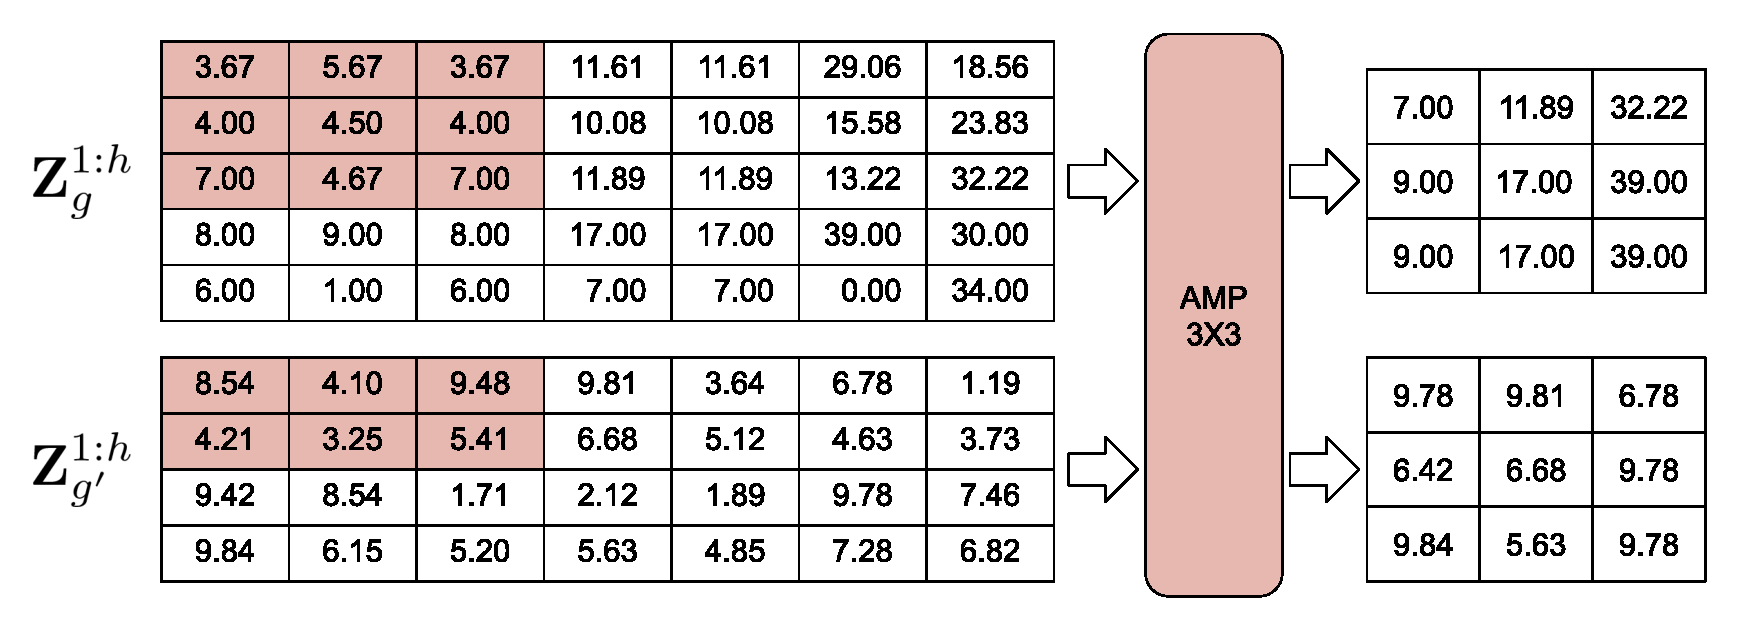
\includegraphics[width=0.90\textwidth]{Magic/figures/ExampleAmp.eps}}
    \caption{Applying AdaptiveMaxPooling Layers to Example Graph $g$}
    \label{MG:Fig:ExampleAmp}
\end{figure*}
